\documentclass[12pt]{article}

\usepackage{sbc}
\usepackage{graphicx,url}
\usepackage{amsmath}
\usepackage[T1]{fontenc}
\usepackage[utf8]{inputenc}
\usepackage[brazil]{babel}

\sloppy

\title{Análise de complexidade do algoritmo Grey Wolf Optimizer\\(Otimização dos Lobos Cinzentos)\\para alinhamento de sequências com uso de discretização para\\aplicabilidade}

\author{Douglas A. C. Canevarollo\inst{1}}

\address{
  Laboratório de Bioinformática\\
  Universidade Estadual Paulista (UNESP)\\Instituto de Biociências, Letras e Ciências Exatas (IBILCE)\\São José do Rio Preto, SP -- Brasil
  \email{douglas.canevarollo@unesp.br}
}

\begin{document}

\maketitle

\begin{abstract}
    Biological sequence alignment is a fundamental problem in bioinformatics, widely used in similarity analysis, evolutionary inference, and protein functional studies. Although exact algorithms such as Needleman–Wunsch guarantee optimal solutions for pairwise global alignment, their computational cost may become significant for larger-scale problems. This work presents a theoretical and experimental complexity analysis of the Grey Wolf Optimizer (GWO), a metaheuristic inspired by the social behavior of grey wolves, adapted to the sequence alignment problem through solution discretization. The asymptotic analysis shows that, for fixed population size and number of iterations, the algorithm exhibits approximately linear time and space complexity with respect to sequence length. To validate this analysis, experiments were conducted using real protein sequences obtained from the UniProt database, evaluating the impact of sequence length, population size, and number of iterations on execution time and memory consumption. The empirical results support the theoretical analysis and indicate rapid convergence during the initial iterations, followed by diminishing returns. The study concludes that discretized GWO provides good scalability and flexibility for obtaining approximate solutions, although it strongly depends on hyperparameter settings and does not guarantee optimality, highlighting the trade-off between computational cost and solution quality.
\end{abstract}

\begin{resumo}
    O alinhamento de sequências biológicas é um problema central em bioinformática, amplamente utilizado na análise de similaridade, inferência evolutiva e estudo funcional de proteínas. Embora algoritmos exatos, como Needleman-Wunsch, garantam soluções ótimas para alinhamento global par-a-par, seu custo computacional pode se tornar elevado em problemas de maior escala. Neste trabalho, realiza-se uma análise teórica e experimental da complexidade do algoritmo Grey Wolf Optimizer (GWO), uma meta-heurística inspirada no comportamento social de lobos cinzentos, adaptado para o problema de alinhamento de sequências por meio de uma discretização das soluções. A análise assintótica mostra que, para tamanho de população e número de iterações fixos, o algoritmo apresenta complexidade temporal e espacial aproximadamente linear em relação ao comprimento das sequências. Para validar essa análise, foram conduzidos experimentos com sequências proteicas reais obtidas da base UniProt, avaliando o impacto do tamanho das sequências, da população e do número de iterações sobre o tempo de execução e o consumo de memória. Os resultados empíricos corroboram a análise teórica e indicam convergência rápida nas primeiras iterações, seguida de retornos decrescentes. Conclui-se que o GWO discretizado oferece boa escalabilidade e flexibilidade para obtenção de soluções aproximadas, embora dependa fortemente de hiperparâmetros e não garanta optimalidade, evidenciando o trade-off entre custo computacional e qualidade da solução.
\end{resumo}

\section{Introdução}

O alinhamento de sequências biológicas é um problema fundamental em bioinformática, com aplicações que incluem a
identificação de similaridade entre genes, inferência filogenética e análise funcional de proteínas. Métodos clássicos,
como o algoritmo de Needleman-Wunsch para alinhamento global \cite{needleman} e o algoritmo de Smith-Waterman para
alinhamento local \cite{smith}, oferecem soluções ótimas baseadas em programação dinâmica, com complexidade de tempo
quadrática $O(nm)$ em relação ao tamanho das sequências $n$ e $m$. Embora a formulação original desses algoritmos também
demande espaço quadrático para a reconstrução do alinhamento, essa limitação já foi superada por Hirschberg
\cite{hirschberg}, cuja técnica de divisão e conquista reduz o espaço necessário para $O(n+m)$ sem comprometer a
otimalidade da solução. A principal restrição prática desses métodos permanece, portanto, o custo quadrático de tempo,
que se torna proibitivo conforme o número e o tamanho das sequências comparadas aumentam.

Diante desse cenário, abordagens baseadas em meta-heurísticas têm sido exploradas como alternativas para lidar com
problemas de otimização de alta complexidade computacional \cite{geraldo}. Resultados na literatura indicam, por
exemplo, que algoritmos inspirados na natureza, como firefly, cuckoo search e flower pollination, conseguem produzir
alinhamentos de boa qualidade com custo computacional linear, superando limitações do Needleman-Wunsch tradicional para
sequências mais longas \cite{shahab}. Entre essas abordagens, destaca-se também o Grey Wolf Optimizer (GWO) \cite{gwo},
um algoritmo inspirado no comportamento social e na estratégia de caça de lobos cinzentos. Originalmente proposto para
problemas contínuos, o GWO tem sido adaptado para domínios discretos, permitindo sua aplicação ao Alinhamento Múltiplo
de Sequências (MSA, do inglês \textit{Multiple Sequence Alignment}) \cite{gwomsa}.

Entretanto, a utilização do GWO nesse contexto levanta questões relevantes quanto à sua eficiência computacional,
especialmente considerando a necessidade de discretização das soluções e o custo associado à avaliação de cada
alinhamento candidato. Embora meta-heurísticas, em geral, ofereçam vantagens em termos de escalabilidade e flexibilidade
para problemas de busca combinatória mais complexos, como o MSA, elas não garantem soluções ótimas, e seu desempenho
tende a depender fortemente de parâmetros como tamanho da população e número de iterações. É justamente esse
compromisso entre flexibilidade e garantias formais que motiva a investigação proposta neste trabalho.

Neste contexto, o presente trabalho tem como objetivo investigar a complexidade de tempo e espaço do algoritmo Grey
Wolf Optimizer aplicado ao problema de alinhamento \textbf{par-a-par} de sequências, considerando uma abordagem baseada
em discretização das soluções. É importante destacar que o alinhamento par-a-par, ao contrário do MSA, já possui
solução exata, ótima e eficiente em tempo e espaço, conforme discutido anteriormente. A escolha desse problema como
objeto de estudo não decorre, portanto, de uma limitação prática do Needleman-Wunsch, mas do interesse em utilizá-lo
como um estudo de caso controlado: por possuir solução ótima conhecida, ele permite avaliar de forma direta os custos e
as limitações de uma meta-heurística -- originalmente concebida para problemas de otimização contínua -- antes de
estender essa discussão a problemas genuinamente intratáveis, como o MSA.

Trata-se, assim, de um trabalho de caráter exploratório, que combina (i) uma análise teórica da complexidade
assintótica de tempo e espaço do GWO discretizado e (ii) uma avaliação empírica de seu desempenho, na qual são medidos
o tempo de execução e o consumo de memória do algoritmo em função do tamanho das sequências, do tamanho da população
(matilha) e do número de iterações. São discutidos, ainda, os principais componentes do algoritmo, sua adaptação ao
domínio discreto e o impacto dessas escolhas de projeto na complexidade computacional resultante.

Por fim, busca-se estabelecer uma comparação entre o GWO discretizado e o algoritmo de Needleman-Wunsch, contrastando
as garantias teóricas de otimalidade e os custos computacionais de cada abordagem. O objetivo não é demonstrar a
superioridade do GWO sobre o método exato -- o que não seria esperado para este problema --, mas sim caracterizar, de
forma quantitativa, os cenários em que o uso de meta-heurísticas pode ser vantajoso, bem como suas limitações,
contribuindo para uma discussão mais ampla sobre os trade-offs entre métodos exatos e aproximados em bioinformática.

\section{Materiais e Métodos}

\subsection{Base de dados proteica}

Para os experimentos, foram utilizadas sequências proteicas reais obtidas a partir da base de dados UniProt \cite{uniprot}. As sequências foram recuperadas programaticamente por meio da API REST do UniProt, restringindo a busca a proteínas humanas manualmente revisadas (\textit{reviewed entries}, Swiss-Prot), correspondentes ao organismo \textit{Homo sapiens} (taxon identifier 9606).

Para cada experimento, foi especificado um comprimento-alvo $n$. A consulta ao UniProt retornou proteínas cujo comprimento pertencia ao intervalo:

\begin{equation}
    [n - 10, n + 10]
\end{equation}

Esse intervalo foi adotado para garantir que as sequências comparadas possuíssem tamanhos semelhantes, reduzindo distorções causadas por diferenças excessivas de comprimento.

Em cada configuração experimental, foram baixadas 10 sequências proteicas, das quais 5 pares distintos foram amostrados aleatoriamente sem reposição. Cada par constituiu uma instância independente do problema de alinhamento.

\subsection{Formulação do problema}

O problema investigado neste trabalho é o alinhamento global par-a-par de sequências proteicas. Dadas duas sequências:

\begin{equation}
    S_1 = s_1s_2\ldots s_n
\end{equation}

e

\begin{equation}
    S_2 = t_1t_2\ldots t_m
\end{equation}

o objetivo consiste em construir um alinhamento global que maximize a similaridade entre ambas, permitindo inserções de gaps para compensar deleções ou inserções evolutivas.

Embora existam algoritmos exatos baseados em programação dinâmica, como Needleman-Wunsch \cite{needleman}, este trabalho utiliza o problema como estudo de caso para análise da complexidade assintótica do Grey Wolf Optimizer (GWO) em um domínio discreto.

\subsection{Grey Wolf Optimizer}

O Grey Wolf Optimizer (GWO), proposto por Mirjalili et al. \cite{gwo}, é uma meta-heurística populacional inspirada na hierarquia social e no comportamento de caça dos lobos cinzentos.

A população é composta por $P$ indivíduos (lobos), cada um representando uma solução candidata. Em cada iteração, os três melhores indivíduos são classificados como:

\begin{itemize}
    \item $\alpha$: melhor solução encontrada;
    \item $\beta$: segunda melhor solução;
    \item $\delta$: terceira melhor solução.
\end{itemize}

Os demais indivíduos atualizam suas posições com base nesses três líderes, seguindo as equações originais do GWO:

\begin{equation}
    \vec{D} = |\vec{C}\cdot \vec{X}{p} - \vec{X}|
\end{equation}

\begin{equation}
    \vec{X}(t+1) = \vec{X}{p} - \vec{A}\cdot \vec{D}
\end{equation}

onde $\vec{A}$ e $\vec{C}$ são vetores de coeficientes aleatórios e $\vec{X}_p$ representa a posição de uma solução líder.

O parâmetro de exploração $a$ decresce linearmente de 2 até 0 ao longo das iterações:

\begin{equation}
    a = 2 - 2\frac{t}{T}
\end{equation}

onde $t$ é a iteração atual e $T$ o número máximo de iterações.

\subsection{Discretização da solução}

Como o GWO foi originalmente proposto para otimização contínua, foi necessária uma adaptação para o domínio discreto do alinhamento de sequências.

Cada lobo foi modelado como um vetor discreto de dimensão:

\begin{equation}
    d = |S_1| + |S_2|
\end{equation}


Cada posição do vetor armazena uma operação de alinhamento pertencente ao conjunto:

\begin{equation}
    \{0,1,2\}
\end{equation}


onde:

\begin{itemize}
    \item 0 representa \textbf{MATCH/SUBSTITUTION};
    \item 1 representa \textbf{GAP em $S_2$};
    \item 2 representa \textbf{GAP em $S_1$}.
\end{itemize}

Após a atualização contínua do GWO, cada nova posição é discretizada por arredondamento:

\begin{equation}
    x' = \operatorname{round}\left(\frac{x_1 + x_2 + x_3}{3}\right)
\end{equation}

O valor discretizado é então limitado ao intervalo válido:

\begin{equation}
    x' \in [0,2]
\end{equation}

garantindo a geração de alinhamentos válidos.

A população inicial foi construída com distribuição enviesada para favorecer alinhamentos biologicamente plausíveis:

\begin{itemize}
    \item 70\% MATCH;
    \item 15\% GAP em $S_2$;
    \item 15\% GAP em $S_1$.
\end{itemize}

Essa estratégia reduz a probabilidade de inicializações excessivamente esparsas em gaps.

\subsection{Função de fitness}

A qualidade de cada alinhamento foi avaliada por uma função de fitness baseada em escore biológico de substituição.

Quando dois aminoácidos são alinhados, sua contribuição é obtida da matriz BLOSUM62 \cite{blosum62}, amplamente utilizada em alinhamento de proteínas por refletir probabilidades evolutivas de substituição.

Assim, para colunas sem gap:

\begin{equation}
    score(i) = BLOSUM62(a_i, b_i)
\end{equation}

Para gaps, foi adotado um modelo de penalidade afim:

\begin{itemize}
    \item Abertura de gap: $-5$;
    \item Extensão de gap: $-1$.
\end{itemize}

Em outras palavras, se um gap é iniciado:

\begin{equation}
    score = -5
\end{equation}

Se o gap continua:

\begin{equation}
    score = -1
\end{equation}

Desta maneira, o fitness total de um alinhamento $A$ é dado por:

\begin{equation}
    f(A)=\sum_{i=1}^{L} score(A_i)
\end{equation}

onde $L$ é o comprimento final do alinhamento.

Como o cálculo exige percorrer toda a representação do lobo, essa etapa domina o custo computacional do algoritmo.

\subsection{Configuração experimental}

A implementação foi realizada em Python, com a utilização de três parâmetros experimentais principais:

\begin{itemize}
    \item $n$: comprimento das sequências;
    \item $P$: tamanho da população;
    \item $I$: número máximo de iterações.
\end{itemize}

Para medir o tempo de execução, utilizou-se a função \texttt{$time.perf\_counter()$}, adequada para medições de alta resolução.

Para medir consumo de memória, utilizou-se o módulo \texttt{tracemalloc}, que registra a memória alocada durante a execução.

Cada configuração foi executada cinco vezes usando pares distintos de proteínas. Os resultados foram agregados por média e desvio padrão.

\subsection{Análise de complexidade}

A análise teórica considera três componentes principais:

\begin{enumerate}
    \item Avaliação de fitness de cada lobo;
    \item Atualização da hierarquia;
    \item Atualização das posições.
\end{enumerate}

A avaliação de fitness percorre toda a representação de um lobo:

\begin{equation}
    O(n)
\end{equation}

Como todos os $P$ lobos são avaliados em cada iteração:

\begin{equation}
    O(P \cdot n)
\end{equation}

A atualização de posições também percorre todos os lobos em todas as dimensões:

\begin{equation}
    O(P \cdot n)
\end{equation}

Portanto, para $I$ iterações, a complexidade temporal total esperada é:

\begin{equation}
    T(n) = O(I \cdot P \cdot n) \label{eq:time_complexity}
\end{equation}

Em relação ao espaço, a estrutura dominante é a população:

\begin{equation}
    P \times (|S_1| + |S_2|)
\end{equation}

resultando em complexidade espacial:

\begin{equation}
    S(n) = O(P \cdot n) \label{eq:space_complexity}
\end{equation}

Os resultados experimentais apresentados na próxima seção foram utilizados para verificar empiricamente a aderência entre essa análise teórica e o comportamento observado na prática.

\section{Resultados e Discussões}

\subsection{Convergência do algoritmo}

A Figura~\ref{fig:convergence} apresenta a curva de convergência do GWO ao longo das iterações.

Observa-se que o fitness da melhor solução cresce rapidamente nas primeiras iterações, partindo de aproximadamente 40 e atingindo valores próximos de 110 em menos de 10 iterações. Após esse ponto, o algoritmo entra em regime estacionário, sem melhorias significativas adicionais.

Esse comportamento indica que o GWO apresenta alta capacidade de exploração inicial, encontrando rapidamente regiões promissoras do espaço de busca. A estabilização precoce sugere que grande parte da otimização ocorre no início da execução, enquanto iterações adicionais contribuem pouco para melhoria da solução.

Tal resultado sugere que, para instâncias de porte semelhante às avaliadas, configurações com menor número de iterações podem reduzir significativamente o custo computacional sem perda substancial de qualidade.

\begin{figure}[ht]
    \centering
    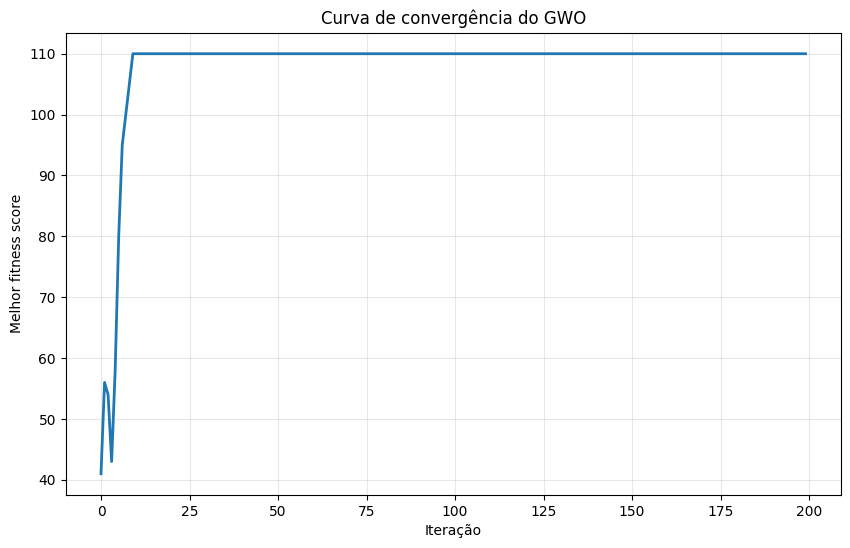
\includegraphics[width=0.75\linewidth]{figures/convergence.png}
    \caption{Curva de convergência do GWO.}
    \label{fig:convergence}
\end{figure}

\subsection{Análise temporal}

A Figura~\ref{fig:time_seq} mostra o tempo de execução em função do tamanho das sequências.

Observa-se crescimento aproximadamente linear no intervalo analisado. Quando o tamanho da sequência aumenta de 25 para 400 aminoácidos, o tempo médio cresce de cerca de 40 segundos para aproximadamente 680 segundos.

Esse comportamento confirma experimentalmente a dependência linear em relação ao tamanho da entrada, consistente com a análise teórica \eqref{eq:time_complexity}, mantendo população e número de iterações constantes.

\begin{figure}[ht]
    \centering
    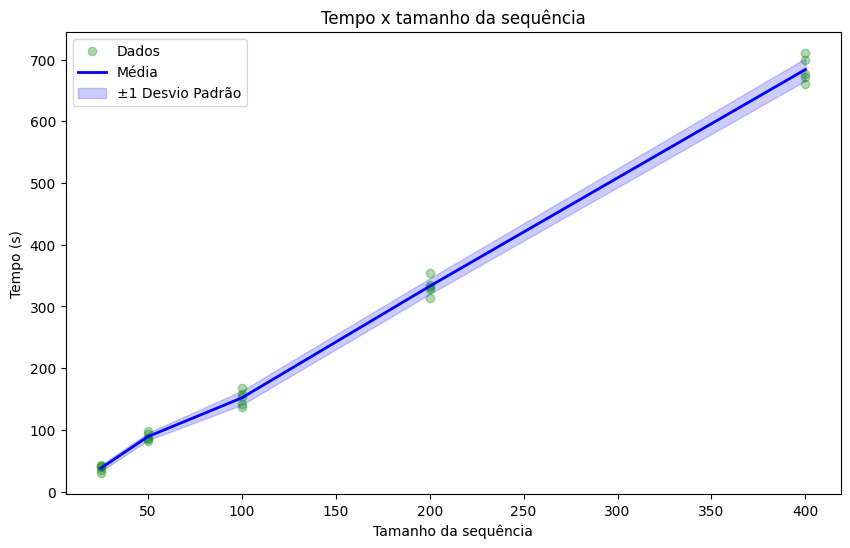
\includegraphics[width=0.75\linewidth]{figures/time-vs-length.png}
    \caption{Tempo de execução em função do tamanho da sequência.}
    \label{fig:time_seq}
\end{figure}

A Figura~\ref{fig:time_pack} apresenta o impacto do tamanho da matilha no tempo total.

O crescimento observado é praticamente linear, validando a hipótese de que o custo por iteração é proporcional ao número de lobos avaliados.

\begin{equation}
    T(P)=O(P)
\end{equation}

Como cada lobo precisa ser avaliado e atualizado a cada iteração, o aumento da população produz impacto direto no custo total.

\begin{figure}[ht]
    \centering
    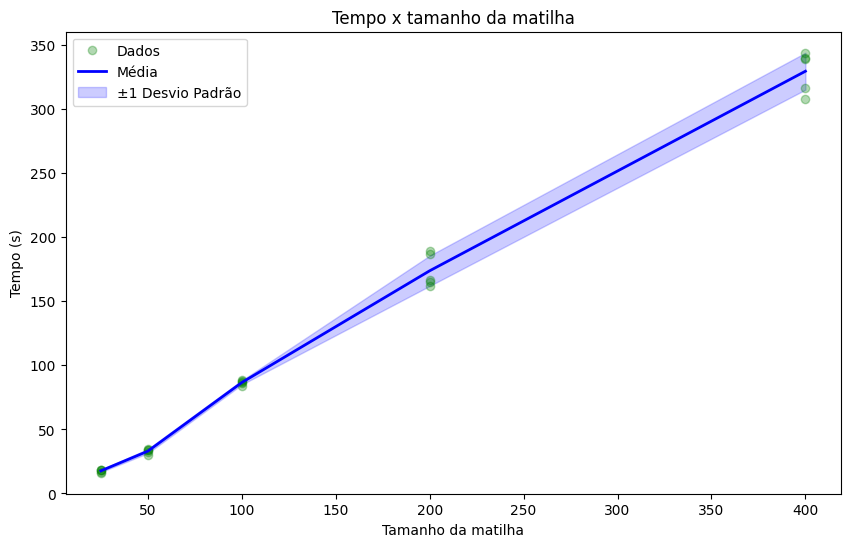
\includegraphics[width=0.75\linewidth]{figures/time-vs-pack.png}
    \caption{Tempo de execução em função do tamanho da matilha.}
    \label{fig:time_pack}
\end{figure}

A Figura~\ref{fig:time_iter} mostra a relação entre tempo e número de iterações.

O crescimento linear observado confirma:

\begin{equation}
    T(I)=O(I)
\end{equation}

Uma vez que cada iteração executa essencialmente o mesmo conjunto de operações, o custo total aumenta proporcionalmente ao número de ciclos de otimização.

\begin{figure}[ht]
    \centering
    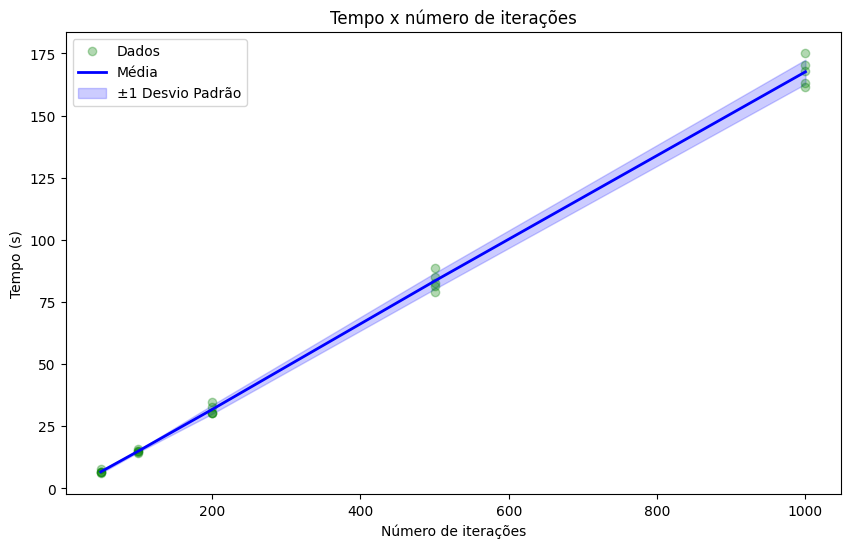
\includegraphics[width=0.75\linewidth]{figures/time-vs-iter.png}
    \caption{Tempo de execução em função do número de iterações.}
    \label{fig:time_iter}
\end{figure}

Em conjunto, os resultados temporais corroboram fortemente a análise assintótica proposta em \eqref{eq:time_complexity}.

\subsection{Análise espacial}

A Figura~\ref{fig:memory_seq} apresenta o consumo de memória em função do tamanho das sequências.

Observa-se crescimento aproximadamente linear, consistente com o fato de que cada lobo armazena uma representação proporcional ao comprimento das sequências \eqref{eq:space_complexity}, quando o tamanho da população é mantido constante.

\begin{figure}[ht]
    \centering
    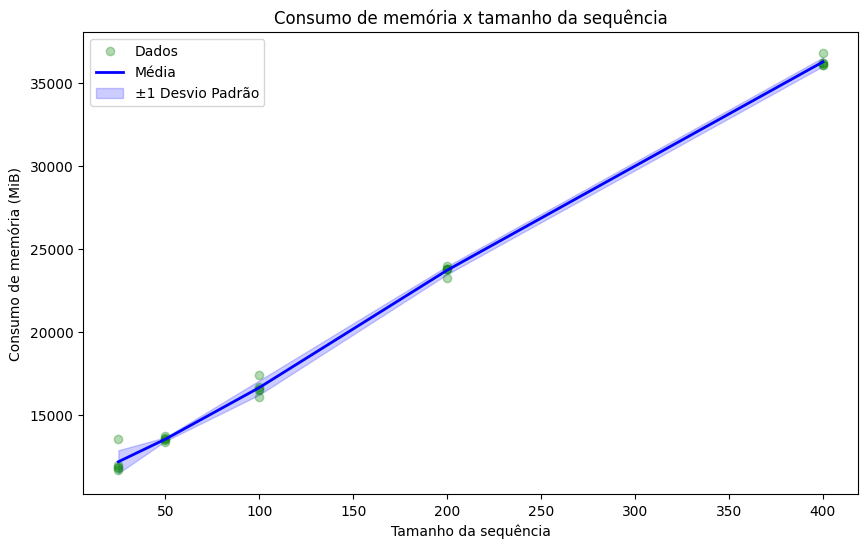
\includegraphics[width=0.75\linewidth]{figures/memory-by-length.png}
    \caption{Consumo de memória em função do tamanho da sequência.}
    \label{fig:memory_seq}
\end{figure}

A Figura~\ref{fig:memory_pack} mostra o impacto do tamanho da população sobre o consumo de memória.

Os resultados indicam crescimento linear, confirmando que a população constitui a principal estrutura de armazenamento do algoritmo.

\begin{equation}
    S(P)=O(P)
\end{equation}

Consequentemente, a complexidade espacial total pode ser descrita por $S(n) = O(P \cdot n)$, conforme definido na equação \eqref{eq:space_complexity}.

\begin{figure}[ht]
    \centering
    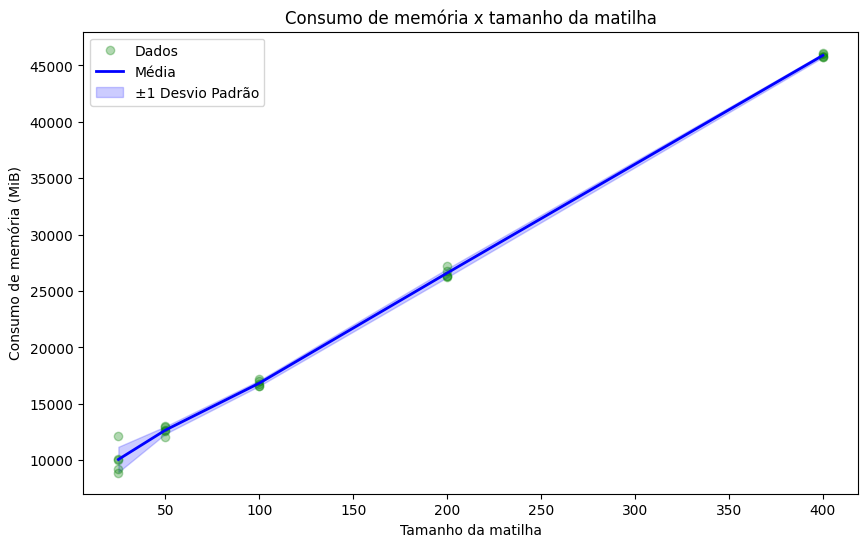
\includegraphics[width=0.75\linewidth]{figures/memory-by-pack.png}
    \caption{Consumo de memória em função do tamanho da matilha.}
    \label{fig:memory_pack}
\end{figure}

\subsection{Discussões}

Os resultados obtidos confirmam empiricamente a análise teórica de complexidade do GWO discretizado para alinhamento de proteínas.

Além da validação assintótica, os experimentos evidenciam um trade-off importante entre custo computacional e qualidade da solução. O aumento do tamanho da matilha melhora a capacidade de exploração do espaço de busca, elevando a probabilidade de encontrar alinhamentos de maior qualidade. Entretanto, esse ganho vem acompanhado de aumento linear no tempo de execução e no consumo de memória.

De forma semelhante, aumentar o número de iterações favorece refinamento adicional da solução, porém com custo computacional proporcional. Como a convergência observada ocorre rapidamente nas primeiras iterações, valores excessivamente altos de iterações tendem a produzir retornos decrescentes.

Em termos práticos, os resultados indicam que o GWO é viável para problemas de pequeno e médio porte, especialmente em cenários nos quais soluções aproximadas de boa qualidade são aceitáveis. Para instâncias muito grandes, o custo computacional acumulado pode tornar métodos exatos ou heurísticas especializadas mais competitivos.

Uma comparação relevante pode ser feita com o algoritmo clássico de alinhamento global de Needleman-Wunsch. Por ser baseado em programação dinâmica, esse método apresenta complexidade temporal de:

\begin{equation}
    O(n \cdot m)
\end{equation}

onde $n$ e $m$ representam os comprimentos das sequências. Para sequências de tamanhos semelhantes, essa complexidade torna-se aproximadamente quadrática:

\begin{equation}
    O(n^2)
\end{equation}

Em contraste, o GWO discretizado analisado neste trabalho apresenta, para população e número de iterações fixos, crescimento aproximadamente linear em relação ao tamanho da sequência \eqref{eq:time_complexity}.

Esse resultado sugere uma vantagem de escalabilidade para o GWO em instâncias maiores. Entretanto, diferentemente de Needleman-Wunsch, que garante a obtenção do alinhamento ótimo global, o GWO produz soluções aproximadas e depende fortemente da configuração de seus hiperparâmetros. Assim, a escolha entre ambas as abordagens depende do trade-off desejado entre optimalidade e custo computacional.

\section{Trabalhos Futuros}

Embora os resultados obtidos tenham validado empiricamente a análise de complexidade do Grey Wolf Optimizer (GWO) discretizado para alinhamento de proteínas, diversas extensões podem ser exploradas em trabalhos futuros.

Uma possível melhoria consiste na \textbf{paralelização do algoritmo}. Como a avaliação de fitness dos lobos é independente dentro de cada iteração, essa etapa é naturalmente paralelizável. Estratégias baseadas em multiprocessamento ou aceleração por GPU podem reduzir significativamente o tempo total de execução, especialmente para populações grandes ou sequências longas.

Outra direção promissora envolve o \textbf{ajuste fino de hiperparâmetros} (\textit{parameter tuning}). Parâmetros como tamanho da população, número de iterações, taxa de exploração e estratégia de inicialização influenciam diretamente o equilíbrio entre qualidade da solução e custo computacional. Técnicas sistemáticas de otimização de hiperparâmetros podem melhorar tanto a convergência quanto a eficiência do algoritmo.

Por fim, uma extensão natural deste trabalho é a aplicação do GWO ao problema de \textbf{alinhamento múltiplo de sequências} (\textit{Multiple Sequence Alignment – MSA}). Diferentemente do alinhamento par-a-par, o MSA envolve simultaneamente múltiplas sequências e apresenta complexidade computacional substancialmente maior, tornando meta-heurísticas populacionais particularmente atrativas. Investigar adaptações do GWO para esse cenário representa uma direção relevante para futuras pesquisas.

\bibliographystyle{sbc}
\bibliography{references}

\end{document}
